\chapter{An introduction to deep learning} \label{chapter2}
Most of our work comprises the design, implementation, and evaluation of deep learning models. This section presents the basics of deep learning models, with a focus on methods for image classification. 

The chapter has been structured, so it can be followed without previous knowledge on machine learning and is based on two canonical manuals in this field: \textit{Deep Learning} \cite{goodfellow2016deep} and \textit{Pattern recognition and machine learning} \cite{bishop2006pattern}. The discussion of specific architectures is based on the excellent \textit{Dive into Deep Learning} course created by Amazon AI professionals \cite{zhang2021dive}.

\section{The basics of neural networks}
Deep Learning comprises a set of machine learning techniques based on the artificial neural networks models. A neural network is composed of units (neurons) connected by links: a link from \( i \) to \( j \) propagates the activation \( a^i \) from \( i \) to \( j \).

Each unit \( i \) receives as input a vector \( x \in \real{n+1} \) where \( x_0 = 1 \) and outputs:
\[ a_i = \varphi \left( w \cdot x\right)\]
the vector \( (w_1, \cdots, w_n) \) is called the vector of \textit{weights} and the term \( w_0 \) is the \textit{bias} of the unit\footnote{We introduce here the one dimensional case, but the adaptation to multidimensional data is straightforward. It must be noticed that neural networks process the data in batches of examples, so the weight tensor has an extra dimension to index the examples.}.

The function \( \varphi: \mathbb{R} \to \mathbb{R} \) is called the activation function, and allows for the appearance of non-linear behavior. The historical choice for the activation function was the Heaviside step function, but it has now been widely replaced by other alternatives, as the logistic function or the sigmoid, which have the advantage of being differentiable.

Neurons can be arranged as an acyclical graph (\textit{feed-forward networks}) or creating a cycle, by feeding the output back to the input (\textit{recurrent networks}). We will focus on the first type of networks, much more common in the \textit{computer vision} field.

Feed-forward networks are arranged in layers: each unit receives input from units in the previous layer. In multilayer neural networks we distinguish input and output layers from the \textit{hidden layers}. The input layer is used to feed information to the network and does not carry any computation, while the output layer is used to produce the final result of the neural network. 

Usually the hidden layers (the ones connecting the input and the output layers) are responsible for carrying out most computational work: its nature and the way hidden layers are connected determine the nature and the learning capabilities of the network. 

\subsection{Universal approximation theorems}
We introduce now some results that should serve to illustrate the power of neural networks: 

\begin{theorem}[Universal approximation theorem \cite{pinkus_1999}]
Let \( \sigma \) be a continuous real function that is not a polynomial. Given \( x \in \mathbb{R}^n \) let \( \sigma \circ x \) denote the element-wise application of \( \sigma \) over the entries of \( \mathbf{x} \).

If \( K \) is a compact subset of \( \mathbb{R}^n \) and \( f \in C(K, \mathbb{R}^m) \) then for every \( \epsilon > 0 \) there exist \( k \in \mathbb{N} \), \( A \in \mathbb{R}^{k \times n},  b \in \mathbb{R}^k, C \in \mathbb{R}^{m \times k} \) such that:
\[ 
    \sup_{x \in K} \| {f(x) - g(x)} \| < \epsilon
\]
where
\[
    g(x) = C \cdot (\sigma \circ (A \cdot x  + b))
\]
\end{theorem}

The previous theorem can be restated more succinctly: the space of functions definable by a neural network with a single hidden layer is dense in \( C(K, \mathbb{R}^m) \) with respect to the topology of uniform convergence. A similar result holds for networks with bounded width and arbitrary depth.

\begin{theorem}[Universal approximation theorem \cite{gripenberg2003approximation}]
Let \( \mathcal{X} \) be a compact subset of \( \mathbb{R}^d \). Let \( \sigma: \mathbb{R} \to \mathbb{R} \) be a non-affine continuous function continuously differentiable with nonzero derivative at least one point. Let \( \mathcal{N}^\sigma_{d, D: d + D + 2} \) denote the space of feed-forward neural networks with \( d \) input neurons, \( D \) output neurons and an arbitrary number of hidden layers each with \( d + D + 2\) neurons with activation function \( \sigma \). Then \( \mathcal{N} \) is dense in \( C (\mathcal{X}, \mathbb{R}^d) \) with respect to the topology of uniform convergence.
\end{theorem}

While these results are useful to showcase the power of neural networks, they have little practical utility. In the first place, their proof is non-constructive, so it leaves open the problem of how can we \textit{train} a given the network to  approximate a given function. The next section offers a high-level review on the topic of training.

In the second place, the theorems provide no assistance on how to define neural networks in practice, where computational resources must be spent wisely. We will address this problem, when discussing the topic of \textit{design} of neural networks for computer vision. 

\subsection{Training of neural networks}
\textit{Training} is the process by which neural networks adjust their parameters to generalize the information obtained from a set of examples, so it can perform accurately on unseen examples. The next paragraphs describe the process of \textit{training} in the context of supervised learning (each example is labelled with the expected output of the net) and using \textit{backpropagation} as the training algorithm. 

During training, neural networks carry out two different processes: forward propagation and backpropagation. During forward propagation, input data is fed to the network in the forward direction in \textit{batches}. For each batch, the hidden layers and the output layer proceed in two steps: preactivation (calculation of the weighted sum of the inputs) and activation (computation of the activation function on the preactivation data). The data resulting from the activation process is fed to the linked units until the output is generated.

The training consist in several epochs, each corresponding to the processing of the whole set through batches. Intermediate results calculated in the hidden layers are preserved, since they will be necessary for the backpropagation.

Once the forward propagation is completed, the loss is calculated by evaluating the loss function \( l \) on the calculated predictions \( \hat{y} \) and the labels \( y \). The regularized loss can be calculated as the sum of the loss and a regularization term:
\[ J = l(\hat{y}, y) + s\]
The regularization term punishes the appearance of large weights or biases, which is useful to prevent overfitting and eases generalization.

The purpose of backpropagation (a process that is only carried during training) is to update the model weights in order to learn from the provided input. To do that, the gradients \[ \frac{\partial J}{\partial W^1}, \frac{\partial J}{\partial W^2}, \cdots, \frac{\partial J}{\partial W^n} \] for each of the weight tensors of the layers are calculated using automatic differentiation which, by the chain rule, implies working in a backwards way.

The opposite of the gradient provides the direction of steepest descent, which is the direction in which the weights must be updated. The \textit{optimization algorithm} chosen determines how the update is carried out.

In \textit{gradient descent}, one of the classics optimization algorithms, the weight \( W \) of each layer is updated to \[ W' = W - \alpha \frac{\partial J}{\partial W} \] where \( \alpha \) is the learning rate.

\begin{figure}[tb]
     \begin{subfigure}[b]{0.49\textwidth}
         \centering
         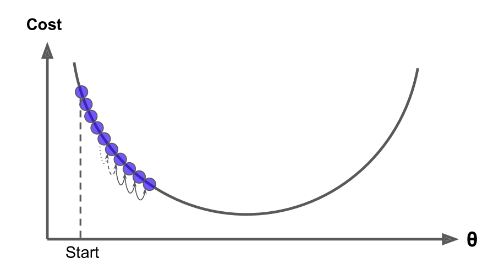
\includegraphics[width=\textwidth]{figures/chapter2/low_lr.png}
         \caption{Low learning rate: slow convergence}
        \label{fig:low_learning_rate}
    \end{subfigure}
    \hfill
    \begin{subfigure}[b]{0.49\textwidth}
         \centering
         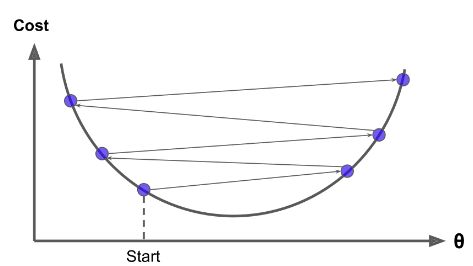
\includegraphics[width=\textwidth]{figures/chapter2/high_lr.png}
         \caption{High learning rate: instability}
         \label{fig:high_learning_rate}
     \end{subfigure}
    \caption{Problems caused by a suboptimal choice of learning rate \cite{geron2022hands}}
    \label{fig:learning_rate}
\end{figure}

The choice of the learning rate becomes crucial, as it is shown in \Cref{fig:learning_rate}: if it is too small, the model will converge very slowly which is computationally inefficient, if it is too high, the learning process will become unstable and the model may fail to generalize. 


Usually calculating the gradient for the entire dataset is computationally unfeasible, so approximations (also dictated by the \textit{optimization algorithm}) are to be used. For example, stochastic gradient descent calculates the gradient from a random subset of the training set.

More complex optimization algorithms (such as Adam \cite{kingma2017adam}) introduce \textit{momentum} (which allows the gradients from previous steps to influence the update of the weights) and adaptive learning rates, reducing the necessity of hyperparameter optimization. 

\section{Convolutional neural networks} \label{sec:cnn}
The universal approximation theorems may lead us to believe that there is no difference between using shallower or deeper neural networks. This belief may be reinforced by the \textit{no free lunch theorem}, which states that “any two optimization algorithms are equivalent when their performance is averaged across all possible problems" \cite{wolper1997freelunch}. While reasonable, this belief is false: in most tasks, deeper networks generalize better, show less overfitting and require an exponentially lower number of training parameters and sample complexity to obtain the same results as shallower nets \cite{hrushikesh2017deep}.

The field of \textit{deep learning} concerns the creation of deep neural networks, with several hidden layers. While deep learning techniques have been known for decades (the theoretical basis were outlined in the 60s) they became widely used around 2012 when several breakthroughs proved modern hardware (especially GPUs) and optimizations had made possible to train big networks that outperformed previous models.

The creation of \textit{deep networks} for image recognition tasks is, however, not straightforward as they present singular problems that make conventional neural networks perform poorly. The first problem is that images are a relatively large type of input, so networks that process images must be wide and have a high number of processing units which makes densely connected layers impractical.

Let's suppose we have as input an image represented as a matrix of pixels \( \mathbf{X}_{i,j} \) and a hidden representation \( \mathbf{H}_{i,j} \), representing the output of the first hidden layer. If we wanted each hidden unit to receive input for each pixel, the matrix of weights should be a 4-dimensional tensor \( \mathbf{W}_{i, j, k, l} \) so that the output of the given layer is (ignoring for the moment the activation function):
\[  \mathbf{H}_{i,j}  = \mathbf{B}_{i, j} + \sum_{k} \sum_{l} \mathbf{W}_{i, j, k, l} \mathbf{X}_{k, l} \]
where \( B \) represents the matrix of biases.

This implies that a network capable of processing a squared image of dimensions \( n \times n \) should have more than \( n^4 \) parameters just in the first hidden layer, far beyond current computational capacity even for small images.

The problem can be alleviated by noticing that most information in images is \textit{translation invariant}: the interpretation of a feature is not dependent on its precise location in the image. This implies the weights and biases of processing units should not depend on the position of the pixel \( i, j \), which allows us to simplify the output of the hidden layer as:
\[  \mathbf{H}_{i,j}  = b + \sum_{k} \sum_{l} \mathbf{W}_{k, l} \mathbf{X}_{k, l} \]

If we re-index by using substitutions \( k = i + a \), \( l = j + b \) (note that \( a \) and \( b \) take both positive and negative values) and introduce \( \mathbf{V} \) such that \( \mathbf{V}_{a, b} = \mathbf{W}_{k, l} \) then the previous equality can be rewritten as:
\begin{equation} \label{eq:convolution}
    \mathbf{H}_{i, j} =  b + \sum_a \sum_b \mathbf{V}_{a,b} \mathbf{X}_{i + a, j + b} = b + V \ast X
\end{equation}
where \( \ast \) is defined as the \textit{convolution} of \( V \) and \( X \).\footnote{Properly speaking, if we interpret \( V \) and \( X \) as multidimensional functions that are \( 0 \) everywhere except in the finite set of indexes of the matrix, then its convolution (in the usual definition) would be given by \( \sum_a \sum_b \mathbf{V}_{a,b} \mathbf{X}_{i - a, j - b} \), the term in \Cref{eq:convolution} is actually the \textit{cross-correlation}. However, it is common in the field to use both terms interchangeably.}

Information in images is usually \textit{locally structured}, which means correlations with local pixels are in general informative, but correlations with remote pixels are usually spurious. This implies we can assume \( \mathbf{V}_{a,b} = 0 \) if \( |a| > \Delta \) or \( |b| > \Delta \) for a certain \( \Delta > 0\). 

The matrix \( V \) is called the \textit{kernel} of the convolution and \( \Delta \) is the size of the kernel. Usually \( \Delta \leq 10 \), so the kernel is much smaller than the original image what makes convolution dramatically more efficient than dense matrix multiplication. 

We consider in \Cref{fig:verticalEdge} an example explaining a convolution between a $6\times6$ image and a $3\times3$ kernel. Our original image has values representing light on the left and null values on the right separated by a vertical axis. We are interested in applying a vertical edge detection kernel in order to detect the axis corresponding to the transition. If we apply the \Cref{eq:convolution} with $b=0$, the obtained matrix represents the vertical axis obtained.
\begin{figure}[tb]
    \centering
    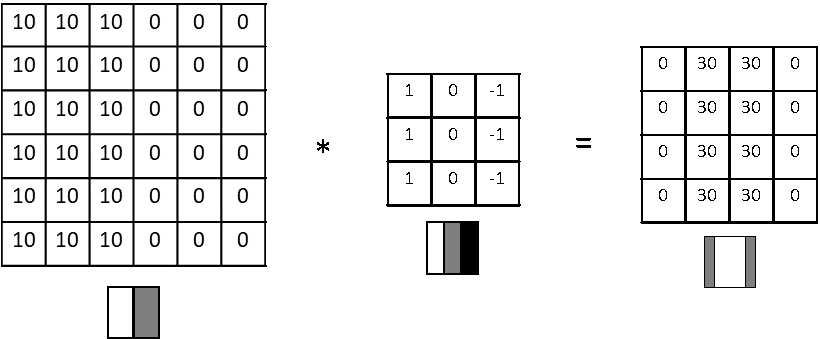
\includegraphics[scale = 0.80]{figures/chapter2/verticalAxis.png}
    \caption{Vertical edge detector example \cite{verticalEdge}.}
    \label{fig:verticalEdge}
\end{figure}

For example, the $H_{0,0}$ element is result of the operation:
\[H_{0,0}=10\cdot 1 + 10\cdot 0 +10\cdot -1+10\cdot 1 + 10\cdot 0 +10\cdot -1+10\cdot 1 + 10\cdot 0 +10\cdot -1=0\]
and the $H_{0,1}$ element is result of:
\[H_{0,1}=10\cdot 1 + 10\cdot 0 +0\cdot -1+10\cdot 1 + 10\cdot 0 +0\cdot -1+10\cdot 1 + 10\cdot 0 +0\cdot -1=30\]

In practice, however, the process of convolution includes some subtleties: since kernels cannot be applied to the peripheral pixels, convolutions usually include \textit{padding} to fill these pixels with \( 0 \) and prevent the input from shrinking through the network. Padding is an important technique since when we do a convolution, the peripheral pixels do not provide the same information as the interior pixels. If we focus on the example of \Cref{fig:verticalEdge} we note that that pixel $X_{0,0}$ is only used to find $H_{0,0}$, while pixel $X_{0,1}$ is used to find $H_{0,0}$ and $H_{0,1}$ and pixel $X_{1,1}$ is used to find $H_{0,0}$, $H_{0,1}$, $H_{1,0}$ and $H_{1,1}$. If we extend the original image by adding 0 valued pixels in the border of the image (\Cref{fig:padding}) the peripheral pixels of the original image have the same importance as the interior pixels, obtaining a more accurate analysis of images. 
\begin{figure}[tb]
    \centering
    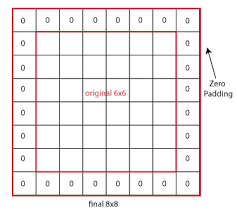
\includegraphics[width=.5\textwidth]{figures/chapter2/zeropadding.png}
    \caption{Zero padding applied to a $6\times 6$ image \cite{paddingImg}.}
    \label{fig:padding}
\end{figure}

There is also the option to skip some intermediate pixels (the \textit{stride}) between convolutions either to save computational resources or to downsample the input. \Cref{fig:Stride} shows a representation of a convolution with stride.
\begin{figure}[tb]
    \centering
    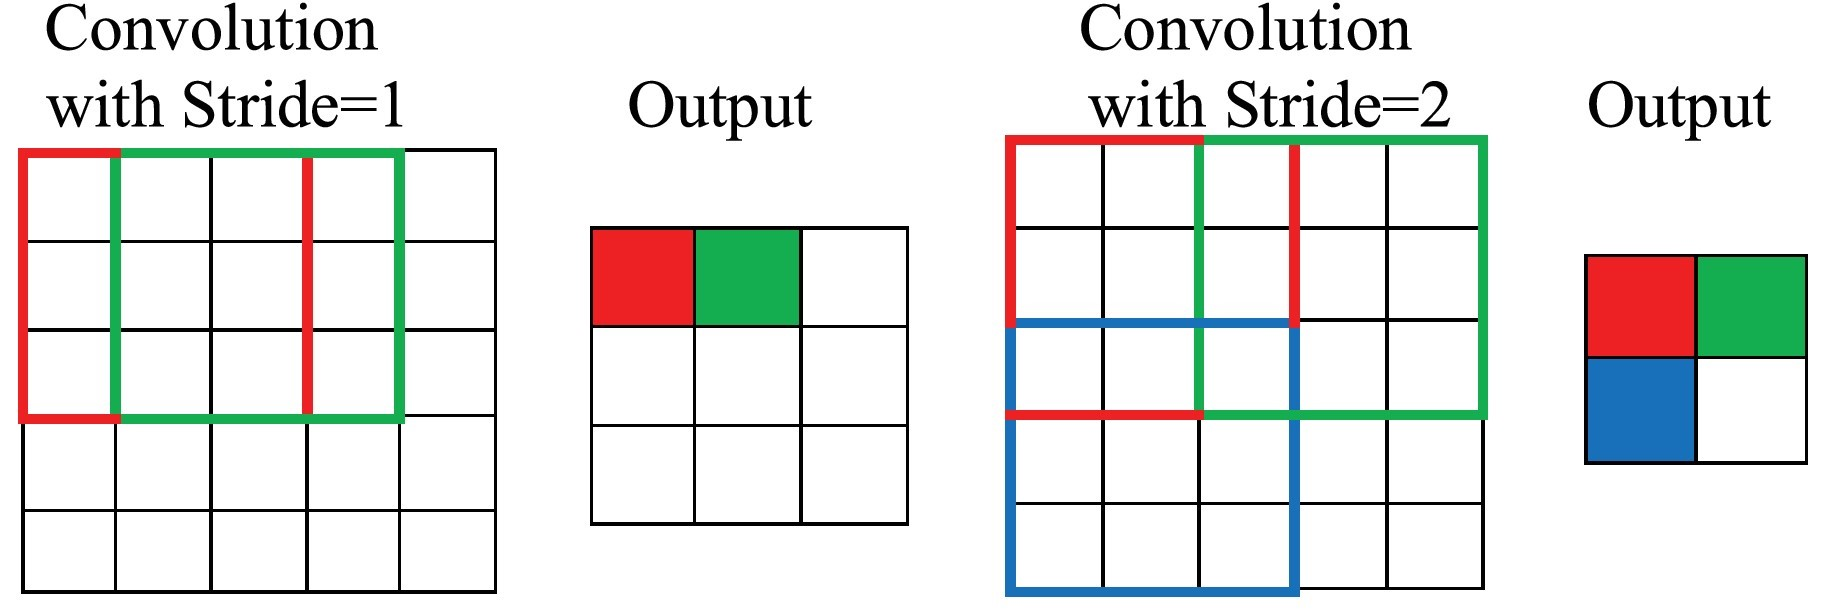
\includegraphics[width=\textwidth]{figures/chapter2/stride.jpg}
    \caption{$1-$Stride and $2-$Stride comparison \cite{strideImg}}
    \label{fig:Stride}
\end{figure}

The application of a kernel allows for the detection of a single feature in many locations. The common practice is to carry out several convolutions in parallel in order to extract multiple features and store each of these features as an output channel. Furthermore, input images usually have multiple channels: for example, one for each of the red, green and blue components. Thus, a hidden convolutional layer computation can be more precisely represented as:
\begin{equation} \label{eq:convolution2}
\mathbf{H}_{i, j, d} = b + \sum_a \sum_b \sum_c \mathbf{V}_{a,b,c,d} \mathbf{X}_{i + a, j + b, c}
\end{equation}
where \( d \) indexes the \textit{output channels} in the hidden representation and \( c \) the image channels\footnote{Since examples are processed in batches, there is another extra dimension to identify each example. We omit it here for the sake of simplicity.}. 

It is common that, as data goes down a convolutional network, the width, and height of the representation shrinks rapidly, while the number of hidden channels, representing the information extracted from each section of the image, grows.

The standard layer of a convolutional network consists of three stages:
\begin{enumerate}
    \item The layer performs several convolutions in parallel to produce a set of linear activations, as described in \Cref{eq:convolution2}.
    \item A nonlinear activation function is computed over each linear activation.
    \item A \textit{pooling function} summarizes local information in a channel by channel basis: for example, by reducing every rectangular neighborhood to the maximum or the average of the neighborhood.
\end{enumerate}

While it is possible to use predefined kernels whose effect is known (for example, edge detection) the standard is to initialize them randomly and train kernels as extra parameter of the model\footnote{This is why in practice we do not need to distinguish between cross-correlation and convolution, as the model will learn the appropriate kernel in each case.}. Classical convolutional networks stack convolutional layers and connect the last layer to a fully connected neural network by flattening it. In the \Cref{fig:archExample} we introduce a $2-$layer convolutional neural network that recognizes a handwritten number from 0 to 9.
\begin{figure}[tb]
    \centering
    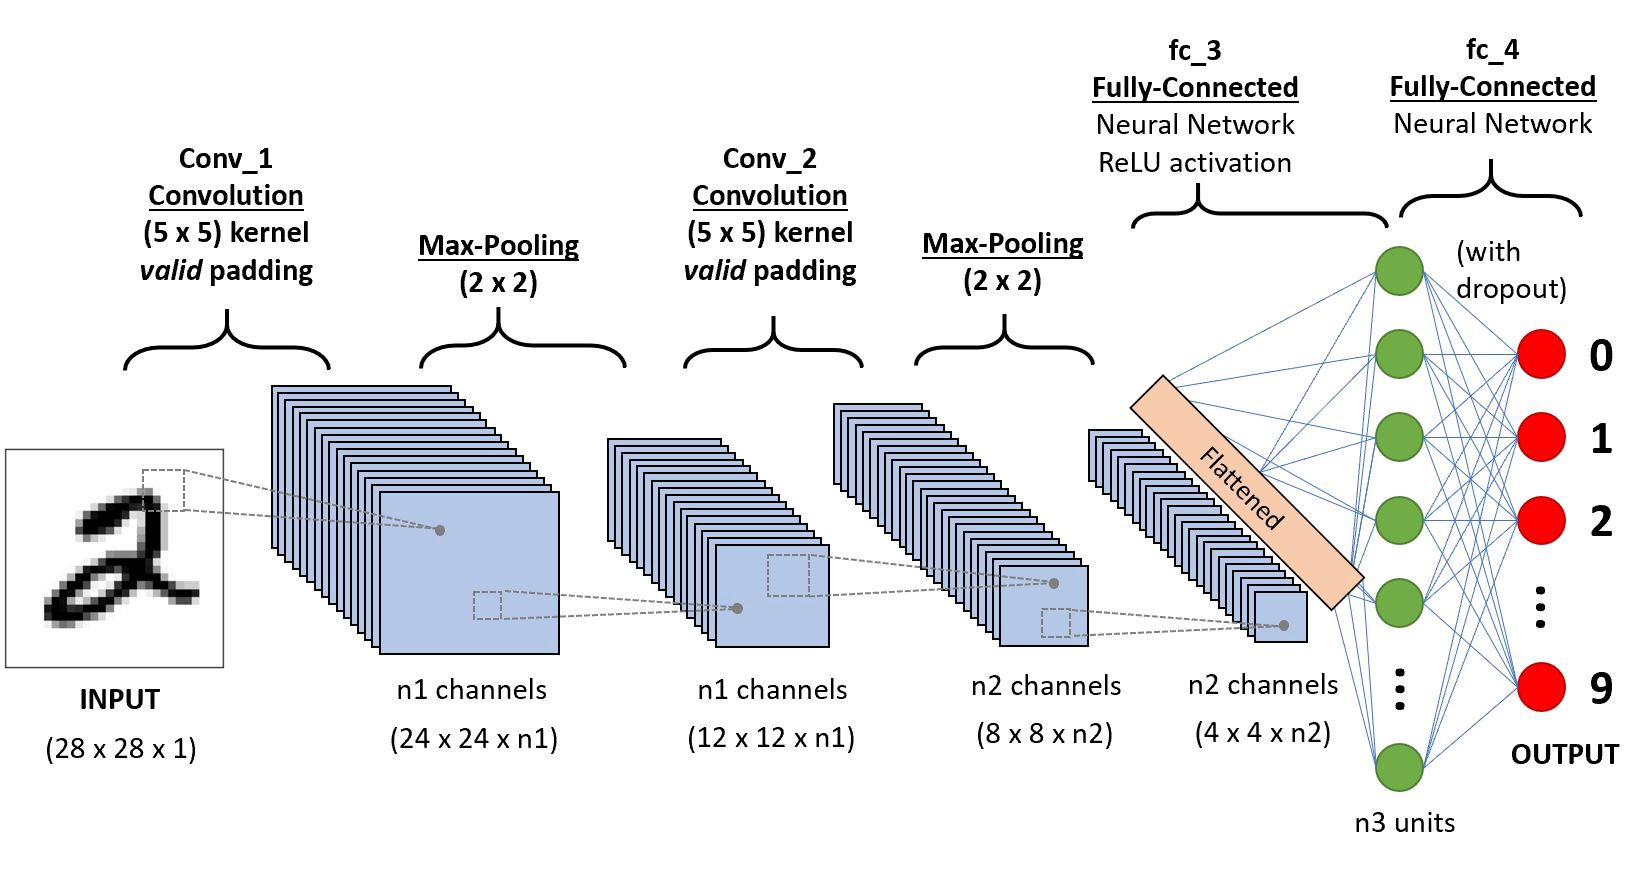
\includegraphics[width=\textwidth]{figures/chapter2/clasicalArch.jpeg}
    \caption{Example of a Convolutional Neural Network that recognizes handwritten digits \cite{classicCNN}.}
    \label{fig:archExample}
\end{figure}

\section{Vision transformers} \label{sec:transformer}
The main alternatives to convolutional neural networks for computer vision problems are vision transformers, a model created for natural language processing problems that was re-adapted for its use on images \cite{vaswani2017attention}. Transformer-based architectures have become the dominant models in natural language processing and other sequence to sequence problem and have been a game-changer in the field of computer vision, having unparalleled scalability on large datasets.

Transformers were created by adapting the \textit{attention mechanism}, common in recurrent neural-networks, to feed-forward networks. The attention mechanism allows the model to revisit the input sequence (for example, a sentence) at every step and selectively focus on parts of the input at particular steps.

\subsection{Attention}
We can understand attention by drawing an analogy to a database, that stores \textit{keys} and \textit{values} that may change through time. This information is used to answer to \textit{queries}. We define the attention over a set of keys and values \( \mathcal{D} = \{ (k_1, v_1), (k_2, v_2) \dots, (k_m, v_m) \)\} for a query \( q \) as:
\[
\attentionop(q, D) = \sum_{i = 1}^m \alpha(q, k_i) v_i
\]
where \( \alpha(q, k_i) \) are scalar attention weights. These weights will determine which elements of the database receive more attention and therefore affect the output the most. Usually weights are normalized (by using the \textit{softmax} function) so they are non-negative and sum to 1: this allows us to interpret the larger weights as selecting the most important components of the input. This means:
\[ \alpha(q, k_i) = \softmax(a(q, k_0), a(q, k_1), \dots, a(q, k_m)) \] where \( a \) is a distance function that will measure similarity between the query and each of the keys. The most commonly used function is \[ a(q, k_i) = q^T k_i / \sqrt{d} \] where \( d \) is the length of the keys, which is particularly convenient to compute as inner products are inexpensive operations. 

Given a set of queries, keys, and values we want the model to combine knowledge in different ways: for example, detecting short-range and long-range dependencies of words inside a sequence. To do that, attention mechanisms are fed \( h \) different independently learned linear projections of the data and the output are concatenated and projected again to produce the final output. This is called \textit{multi-headed attention} and resembles the \textit{pooling} mechanism of convolutional neural networks.

Transformers follow an architecture called \textit{self-attention} that works as follows: first, we create a representation of our input as a sequence of tokens, each token having its own query, keys, and values. This sequence of tokens is fed into the attention mechanism. Each token can pay attention (using its query vector) to other tokens (which it will match using their key vectors). For each token we then create a new representation, that will be fed to the next layer and that potentially includes information from all other tokens. Since each token is connected to every other token, the time complexity of using self-attention on \( n \) tokens with values of length \( d \) is \( \mathcal{O}(n^2 d) \), but since most operations are independent we can carry these computations in parallel, and we only have \( \mathcal{O}(1) \) sequential operations.

The way the data is encoded as tokens (including queries, keys, and values) is usually learned by the model itself. Notice that the encoding usually loses all positional information of the sequence which may be useful later on. To solve this, additional tokens marking the original position of each token in the input sequence are added, a technique known as \textit{positional encoding}.

\subsection{The transformer architecture}
\begin{figure}[tb]
    \centering
    \includesvg[width=.6\textwidth]{figures/chapter2/attention/transformer.svg}
    \caption{The transformer architecture \cite{zhang2021dive}}
    \label{fig:transformer}
\end{figure}

We are ready to introduce the \textit{transformer} architecture, presented in \Cref{fig:transformer}. The \textit{transformer} is a type of \textit{encoder-decoder} architecture: the \textit{input}, of varying length, is transformed through the \textit{encoder} into a fixed size representation, the \textit{state}. The \textit{decoder} will generate the output from this representation.

The \textit{encoder} is a stack of multiple identical layers, where each layer has two sublayers: a multi-head self-attention layer and a position-wise feed-forward network, which transforms the representation of all tokens using the same multi-layer network. Every layer is fed the output of the previous layer. \textit{Residual connections} \cite{he2016deep} and layer normalization are used to ease convergence of the model and prevent misbehaved gradients. 

The \textit{decoder} is also a stack of identical layers, including residual connections and layer normalization. Besides the two first sublayers coincides with the ones described in the encoder, there is a third sublayer, the \textit{encoder-decoder attention}. In this layer, queries come from the output of the previous decoder layer while the keys and values come from the encoder outputs. A \textit{masked attention} mechanism is used, so each position in the decoder can only attend previous positions, so the process of decoding behaves as an \textit{autoregressive} process and only depends on the tokens already generated.

\subsection{Vision transformers} 
\begin{figure}[tb]
    \centering
    \includesvg[width=.8\textwidth]{figures/chapter2/attention/vit.svg}
    \caption{The vision transformer architecture (ViT) \cite{zhang2021dive}.}
    \label{fig:vit}
\end{figure}

Transformers were adapted to computer vision problems in a far-reaching paper that introduced the Vision Transformer (ViT)\cite{dosovitskiy2020image}. The model used a technique called \textit{patch embedding}, consisting on splitting the image as patches and encoding each patch using an encoder architecture. 

A special token \textit{<class>} summarizes the information in the rest of patches (using self-attention). This token is then fed to the classifier, a MLP that will generate the label for the image. 

While the name \textit{vision transformer} initially referred to a concrete model (ViT) the term now refers to a variety of related models as DeiT \cite{pmlr-v139-touvron21a} or Swin \cite{liu2021swin}, which also use attention on patches of the original image.

\section{Vision transformers vs CNNs}
The choice between vision transformers and CNNs must be done carefully and take into account the nature of the problem at hand, the availability of data, the computational resources available, the performance expectations and the interpretability requirements.

While vision transformers scale better with data and are, at the time of writing, the dominant models for big datasets, as ImageNet \cite{imagenet}, for small to medium datasets (thousands of images) CNNs architectures can outperform vision transformers \cite{tan2021efficientnetv2}. The main reason is that transformers design does not incorporate translation invariance or locality, properties that ease convergence on small datasets.

The quadratic complexity of self-attention makes transformer inefficient with high resolution images, although this problem has been addressed by models like Swin \cite{liu2021swin}.

Both reasons make CNNs a natural option to work with medical datasets, which usually are medium-sized and formed by high resolution images. There has been a significant effort to design efficient CNNs architectures, that can be trained with a fraction of the resources necessary for a transformer \cite{tan2021efficientnetv2}.

However, vision transformers have excellent interpretability properties \cite{chefer2021transformer} because attention can be visualized to determine which parts of the image are driving the classification. 

As we argued previously, our limited computational resources made us opt for convolutional neural networks as the backbone of our solution, although we explore and discuss other alternatives. 

\section{Interpreting vision models} \label{seq:transformer}
Interpretation of neural networks present several significant challenges. Most neural networks behave as \textit{black-box} models: they return a result without explaining how they arrived at that conclusion. The nature of deep neural networks makes them hard to interpret, since the hidden representations the network learns usually has no evident connection with the original data.

However, there exist different techniques for \textit{interpreting} a model, differing on the way they work and the result they produce (a heatmap of the most relevant parts of the image, a segmentation of the factors boosting classification…). These techniques may be either model specific or model agnostic. 

Model specific techniques exploit details about the model architecture to extract information about their performance. For example, for CNNs we can visualize the learned kernels for some convolutional layers. 

These techniques are usually the most expressive, as they include information about the model design. However, they are bound to a certain architecture and therefore cannot be used to interpret the performance of different architectures.

Model agnostic techniques do not make assumptions about the structure of the model. For example, they may include small perturbations of the input and analyze the variation of the output. There exist different variations of this technique: for example, learning a linear model on the vicinity of an instance we want to explain that is locally similar to the model \cite{lime} or using techniques from game theory to allocate \textit{credibility} to different features \cite{lundberg2017unified}.

It must be emphasized that these techniques do not reproduce the way the model works, they just be interpreted as an \textit{intuition}. This means, for example, that they should not be used as the main method to evaluate the performance of a model, and it is best to contrast the result from multiple techniques. In second place, interpretability techniques can only offer so much intuition about the performance of a generic model. Interpretable models must be designed with this idea in mind, which usually require general architectural changes and may require sacrificing performance or efficiency.